\documentclass{article}
\usepackage{graphicx}
\usepackage[utf8]{inputenc}
\usepackage[T1]{fontenc}
\usepackage{makecell}
\usepackage{subfig}
\usepackage{diagbox}
\usepackage{needspace}
\usepackage{hyperref}
\usepackage{amsmath}
\usepackage[dvipsnames]{xcolor}
\usepackage[polish]{babel}
\usepackage[a4paper,
            left=1in,
            right=1in,
            top=1in,
            bottom=1in]{geometry}
\usepackage{selinput}
\usepackage{amsmath,amssymb}
\SelectInputMappings{
  cacute={ć},        
  lslash={ł}
}
\usepackage{listings}
\usepackage{color}
\usepackage{gensymb}

\definecolor{dkgreen}{rgb}{0,0.6,0}
\definecolor{gray}{rgb}{0.5,0.5,0.5}
\definecolor{mauve}{rgb}{0.58,0,0.82}

% \newcommand{\code}[1]{\textcolor{Fuchsia}{\textbf{\texttt{#1}}}}
\renewcommand{\contentsname}{Spis treści}
\addto\captionspolish{\renewcommand{\refname}{Źródła}}

\renewcommand*\descriptionlabel[1]{\hspace\leftmargin$#1$}
\addto\captionspolish{\renewcommand{\figurename}{Zdjęcie}}

\title{%
    Zadanie rekrutacyjne do KN Solvro\\
    \large{Sekcja uczenia maszynowego}
}
\author{Krzysztof Głowacz}
\date{wiosna 2025}

\makeatletter         
\def\@maketitle{
\raggedleft

\includegraphics[height = 15mm]{logo.png}\\[8ex]
\vspace{1.5cm}
\begin{center}
{\Huge \@title }\\[6ex]
{\Large  \@date}\\[15ex]
{\Large  \@author}\\[40ex]
\end{center}}
\makeatother

\lstset{frame=tb,
  language=Python,
  aboveskip=3mm,
  belowskip=3mm,
  showstringspaces=false,
  columns=flexible,
  basicstyle={\small\ttfamily},
  numbers=none,
  numberstyle=\tiny\color{gray},
  keywordstyle=\color{blue},
  commentstyle=\color{dkgreen},
  stringstyle=\color{mauve},
  breaklines=true,
  breakatwhitespace=true,
  tabsize=3
}

\definecolor{light-gray}{gray}{0.95}
\newcommand{\code}[1]{\colorbox{light-gray}{\texttt{#1}}}

\begin{document}

\maketitle
\tableofcontents
\clearpage

\section{Wstęp}
    W niniejszym raporcie przedstawione zostało rozwiązanie zadania rekrutacyjnego do sekcji uczenia maszynowego Koła Naukowego Solvro (rekrutacja wiosenna 2025). Zadanie polegało na eksploracyjnej analizie danych oraz klasteryzacji podanego zbioru \cite{instrukcja}.

\section{Analiza danych}
    Zbiór danych, pochodzący z bazy danych TheCocktailDB, zawierał listę koktajli wraz ze składnikami niezbędnymi do ich przyrządzenia. Link do zbioru danych został dołączony do sekcji Źródeł tego raportu \cite{zbior_danych}.

    Pierwsza analiza zbioru danych wykazała, że konieczna będzie osobna analiza składników koktalji, które początkowo były reprezentowane jako zagnieżdżone struktury danych wewnątrz rekordów opisujących koktajle. W celu przeprowadzenia poprawnej wstępnej analizy danych (\textit{EDA}) napisany został skrypt \code{src/eda.py}, który miał za zadanie:
    \begin{itemize}
        \item wczytać dane z pliku w formacie JSON do formatu DataFrame z biblioteki Pandas,
        \item wydzielić dane dotyczące składników koktajli do osobnego DataFrame'a,
        \item wyświetlić podstawowe statystyki danych,
        \item wygenerować pełne raporty opisujący dane o koktajlach i składnikach koktajli korzystając z biblioteki ydata-profiling.
    \end{itemize}
    Na zdjęciu nr \ref{fig:run_eda} przedstawiony został fragment wyjścia standardowego po uruchomieniu skryptu.

    \begin{figure}[!htbp]%
        \centering
        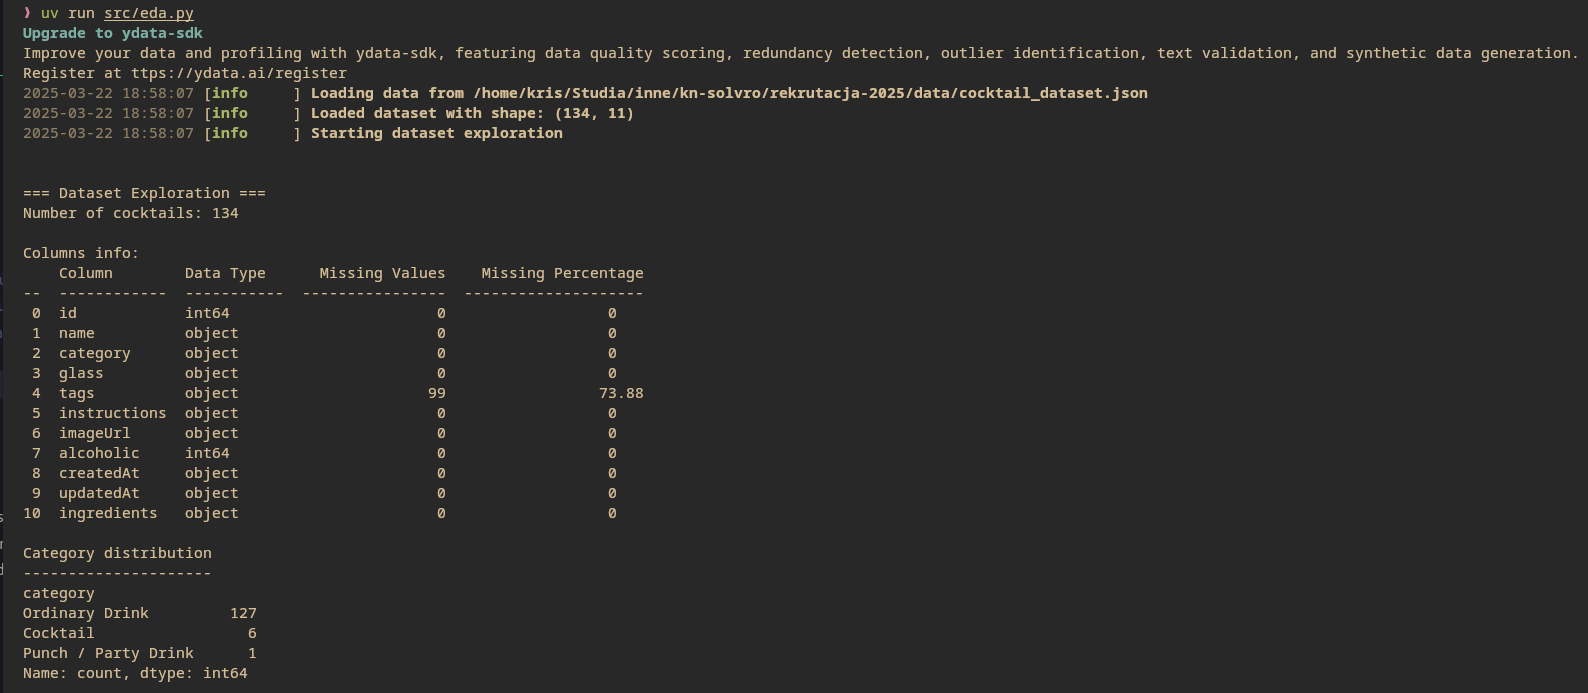
\includegraphics[width=\textwidth]{eda_run.png}
        \caption{Uruchomienie skryptu src/eda.py}%
        \label{fig:run_eda}
    \end{figure}

    Informacje dostarczone przez skrypt i wygenerowany raport pozwoliły na wyciągnięcie nastepujących wniosków:
    \begin{enumerate}
        \item Każdy koktajl ze zbioru danych opisany jest przez 11 cech, przy czym 4 z nich są zupełnie nieistotne z punktu widzenia dalszej analizy, ponieważ albo zawierają informacje typowo bazodanowe (kolumny: \textit{id}, \textit{createdAt}, \textit{updatedAt}), albo są linkiem URL do zdjęcia przedstawiającego dany koktajl (\textit{imageUrl}). Cecha \textit{tags} także została na tym etapie odrzucona - niespełna 74\% koktajli nie ma żadnego tagu przypisanego, a gdy koktajl ma przypisane tagi to sprawiają one wrażenie bardzo luźno powiązanych, niezbyt informatywnych. Cecha \textit(instructions) także została odrzucona, ponieważ zawiera ona opis przygotowania koktajlu w języku naturalnym, co nie stanowiło dobrej podstawy do późniejszej klasteryzacji.
        \item Cecha \textit{category} jest mało wartościowa w kontekście późniejszej klasteryzacji ze względu na fakt, że zawiera jedynie 3 różne wartości, przy czym zdecydowana większość koktajli ma przypisaną taką samą kategorię (Ordinary Drink - zdjęcie \ref{fig:category}).
        \item Cecha \textit{alcoholic} jest nieistotna ze względu na to, że przyjmuje stałą wartość równą 1 (tzn. wszystkie drinki są alkoholowe).
        \item Jedyną cechą składników koktajli łatwą do uwzględnienia w późniejszej klasteryzacji była ich alkoholowość, tzn. flaga informująca o tym, czy dany składnik zawiera alkohol.
    \end{enumerate}

    \begin{figure}[!htbp]%
        \centering
        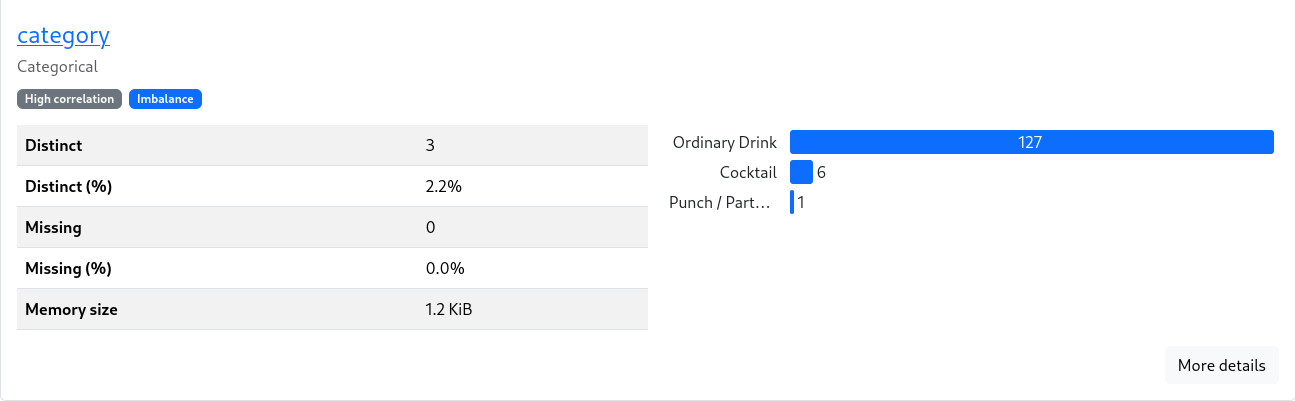
\includegraphics[width=\textwidth]{category_eda.png}
        \caption{Analiza cechy \textit{category}}%
        \label{fig:category}
    \end{figure}


\section{Przygotowanie danych}
Ciekawym pomysłem na poradzenie sobie z zagnieżdżoną strukturą składników koktajli była prosta ich agregacja - przypisanie do każdego koktajlu łącznej liczby składników, liczby składników zawierających alkohol i tych bez alkoholu.
Następnie usunięto z DataFrame'u niepotrzebne kolumny (opisane w poprzedniej sekcji).

Kolejnym etapem przygotowania danych było ich enkodowanie - zastosowano \code{LabelEncoder} na kolumnie \textit{glass}. Ostatnim krokiem tego procesu było przeskalowanie danych przy pomocy \code{StandardScalera}.


\section{Klasteryzacja}
Do wyznaczenia liczby klastrów użyto \textit{Elbow Method}, która wskazywała na 4 lub 5 klastrów. Przyjęto wartość 4 ze względu na stosunkowo mały zbiór danych. Dane zostały sklasteryzowane metodą \code{KMeans} z biblioteki \textit{scikit-learn}. Wykres ze zdjęcia \ref{fig:results} prezentuje efekty klasteryzacji.

Widoczny jest podział koktajli względem łącznej liczby potrzebnych składników, a także względem alkoholowych składników. Możemy wyróżnić 4 grupy koktajli:
\begin{itemize}
    \item te, które wymagają tylko 1 składnika alkoholowego oraz niewielu składników sumarycznie (2/3/4).
    \item te, które wymagają niewielu składników alkoholowych (1/2) oraz wielu składników sumarycznie (5/6).
    \item te, które wymagają kilku składników alkoholowych (2/3) przy jednoczesnej niewielkiej liczbie sumarycznych składników (2/3/4).
    \item te, które wymagają wielu składników alkoholowych (2/3/4) i wielu składników sumarycznie (5/6).
\end{itemize}

\clearpage

\begin{figure}[!htbp]%
    \centering
    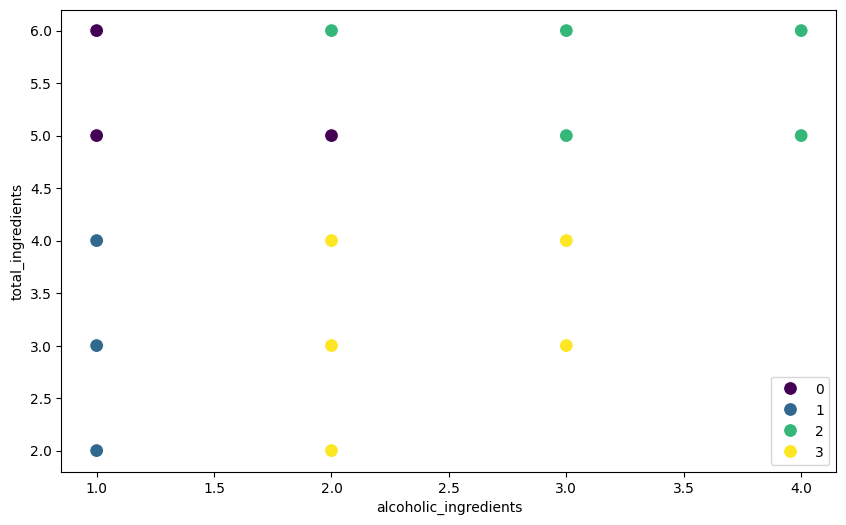
\includegraphics[width=\textwidth]{clusters.png}
    \caption{Efekt klasteryzacji}%
    \label{fig:results}
\end{figure}

Można się zgodzić, że dokonany podział jest zasadny i stosunkowo logiczny. Poza ewaluacją jakościową przeprowadzono także ewaluację ilościową i otrzymano następujące wartości metryk:\\
\begin{table}[!htbp]%
    \centering
    \begin{tabular}{l|r}
        Metryka & wartość \\ \hline
        Inertia & 324.19 \\
        Silhouette Score & 0.3119 \\
        Calinski-Harabasz Score & 46.22 \\
        Davies-Bouldin Score & 1.3301 \\
    \end{tabular}
\end{table}\\


Na ich podstawie możemy stwierdzić, że dokonana klasteryzacja, nawet bez odpowiedniego tuningowania hiperparametrów okazała się całkiem skuteczna, co potwierdziły przeprowadzone ewaluacje.

\vspace{1cm}
\hrulefill
\bibliographystyle{plain}
\bibliography{references}
\end{document}
